\section{\odlib}
\label{sec:od}


% \todo{perhaps offer a list of libraries available to give a feel?}
In this section, we 
describe \odlib, a framework that allows developers to easily design, measure and deploy replication protocols over modern hardware.
Specifically, \odlib~contains libraries to perform, among other things, the following:
create and pin software threads, initialize and interface with the KVS, initialize RDMA data structures, exchange \RDMA~metadata to connect the servers, send and receive \RDMA~messages, initialize and use the \RDMA~multicast primitive, detect failures and maintain the configuration, specify and implement the read/write API (or create traces for benchmarking) and finally measure the performance of the system. % (throughput and latency). 

All \pnum~of our protocols are implemented over \odlib.
Therefore, describing \odlib~serves a dual purpose: presenting implementation details of our evaluated protocols and describing how \odlib~can be used by the community to design and deploy new protocols.

In the rest of this section we first describe the utility of \odlib\ (\S\ref{sec:why}), and then focus on its three basic components: the threading model (\S\ref{sec:ex-mod}), the Key-Value Store layer (\S\ref{sec:kvs}) and the networking layer (\S\ref{sec:nw}).
% and the generic API (\S\ref{sec:api}). %For each of the components we will describe the developer involvement required to use the features.

% Specifically, \odlib~contains libraries to perform the following (not an exhaustive list):
% create and pin software threads, initialize and interface with the KVS, initialize RDMA data structures, exchange \RDMA~metadata to connect the servers, send and receive \RDMA~messages, initialize and use the \RDMA~multicast primitive, detect failures and maintain the configuration, specify and implement the read/write API (or create traces for benchmarking) and finally measure the performance of the system (throughput and latency). 
\subsection{Utility of \odlib}\label{sec:why}
% \todo{1. modern hardware for performance, 
% 2. it's very hard to do, tricky and time consuming 
% 3. for hermes, farm it took this much time }

The utility of \odlib~is twofold. Firstly, for the purposes of this paper, it allows us to compare strongly-consistent replication protocols over modern hardware.
Secondly, once open-sourced, \odlib\ can be used to develop new (or old) protocols over modern hardware.
Below, we elaborate on why \odlib\ is necessary to achieve either of these goals.
%is crucial in achieving both goals 
% and then briefly describe a case-study of using \odlib. 
% In \secref{sec:related}, we explain why existing solutions were not sufficient for our purposes.


\beginbsec{Protocol comparison}
\odlib\ facilitates an apples-to-ap\-ples comparison between strongly-consistent replication protocols over modern hardware:
% Firstly, note that by using \odlib, we ensure a fair comparison: 
all our protocols use the same threading model, underlying KVS and networking patterns and optimizations.
However, it is not enough for the comparison to be fair; it must also be meaningful. For that, protocols must be able to stress modern hardware to its limits. Only then will the protocol inefficiencies be exposed.
For instance, \figref{fig:single-thr}, orders our \pnum\ protocols by their single-threaded performance;
this order changes drastically when multi-threading them in \figref{fig:write-all}. 
This is because multi-threading stresses the hardware, which in turn exposes protocol pathologies. % (e.g. lack of thread-scalability).
The need to stress the hardware necessitates a framework, such as \odlib, that targets multi-threaded, \RDMA-enabled, in-memory KVSes.


\beginbsec{Development of new protocols}
The second purpose of \odlib\ is to accelerate the development and deployment of replication protocols over modern hardware.
Note that in most of our protocols 80 to 90\% of the codebase is devoted to tasks such as %pinning software threads and 
setting up and using the KVS and the RDMA networking.
The challenge is that, while orthogonal to protocol design, these tasks 
require intimate domain-specific knowledge.

To get a taste of what this knowledge entails, let us look at a specific example of a commonly occurring error when using RDMA.
Assume that an \RDMA~message that appears to have been transmitted is never received.
Also assume 
the developer is wise enough to check the hardware counters and detects that \emph{req\_cqe\_error} has been incremented.
In that case, the developer must know from experience that the most likely cause for this error is attempting to send a message from a memory location that has not been registered with the NIC. Absent that intimate knowledge of the RDMA universe, the developer would have to make due
with the manual's enigmatic explanation, that a \qt{completion queue event has completed with an error}~\cite{Mellanox:2020}.

\odlib\ frees the developer from all that cumbersome complexity allowing them to focus solely on the protocol. Under the hood, \odlib\ uses best practices and optimizations from different domains
% , leveraging years of research, 
to maximize performance.
% The developer is now free to focus solely on designing their protocol.

%\beginbsec{A case-study} 
To get a better sense of \odlib's utility, let us consider a concrete example in the form of 
Hermes over \odlib.  Was development accelerated? It took one developer less than 2 working days to develop and test our \odlib-based Hermes. Did \odlib\ practices help performance?
%Firstly, 
%Furthermore, 
Our \odlib-based Hermes enjoys a 20\% increase in write throughput, compared to the open-sourced version. We attribute the increase to \odlib's \emph{smart messages} (explained in \secref{sec:nw:sm}).
% Using the \odlib~library, 
%and by reusing code from similar functionality implemented in our other protocols, 
% . 
% Leaning into the expertise embedded in \odlib\ also paid off:
% our \odlib-based Hermes enjoys a 20\% increase in write throughput, compared to the open-sourced version, which we attribute to \emph{smart messages}, an optimization we explain in \secref{sec:nw:sm}.

%years of expertise under the hood, allowing the developer to exercise their own years of expertise in designing their protocols.

\begin{comment}


The challenge in developing a protocol with \odlib~like features, is that it requires intimate domain-specific knowledge in areas orthogonal to protocol design. Pinning software threads, setting up and using the KVS and the RDMA networking, creating measuring tools are examples
In fact, in most of our protocols 80 to 90\% of codebase is devoted to such tasks. Protocol code only takes up 

to c tasks such as as RDMA networking, KVS
Developing even the simplest protocol is very challenging, because it requires 

Problematically, only 10\% of Hermes codebase is devoted to implementing the protocol. The rest 90\% performs various other tasks such as creating and pinning software threads or setting up and using the KVS and the RDMA networking.
Crucially, these tasks often
require intimate domain-specific knowledge.

To get a taste of what this knowledge entails, let us look at a specific example of a commonly occurring error when using RDMA.
Assume that an \RDMA~message that appears to have been transmitted is never received.
Also assume 
the developer is wise enough to check the hardware counters and detects that \emph{req\_cqe\_error} has been incremented.
In that case, the developer must know from experience that the most likely cause for this error is attempting to send a message from a memory location that has not been registered with the NIC. Absent that intimate knowledge of the RDMA universe, the developer would have to make due
with the manual's enigmatic explanation, that a \qt{completion queue event has completed with an error}~\cite{Mellanox:2020}.

Designing a protocol that can be explained in a few sentences should be done in a few hundreds lines of code
It is particularly challenging attempting to solve is the difficulty of developing, and deploying a replication protocol over modern hardware.
The difficulty stems from the fact that 

purpose of \odlib\ is to allow the community to easily develop and test new protocols for modern hardware.



wh
of our \pnum~protocols when single-threaded. 
\figref{fig:single-thr} and~\ref{fig:write-all} exemplifies this, by  showing that protocols by multi-threading protocols, their relative performance changes radically.

to draw meaningful insights we must implement the protocols over modern hardware: heavily multi-threaded,

comparison must not only be fair, but 
E

A new infrastructure is necessary to perform the comparison because 1) open-source implementations are typically not built for modern hardware.
Furthermore, 


Most importantly they are typically single-threaded and not RDMA-enabled.

Instead, \odlib~protocols are heavily multi-threaded leveraging modern parallel hardware, they are RDMA-enabled, leveraging best practices established over the last decade, and uses an in-memory state-of-the-art KVS. 

The combined difference between a single-threaded, TCP-based replicated KVS and a multi-threaded, RDMA-enabled one is roughly two to three orders of magnitude. 
For example, the throughput of \odlib~based protocols is on the millions per second.
Conversely, their counterparts, when built using Paxi~~\cite{Ailijiang:2019}, a similar system to \odlib, but single-threaded and TCP-based, are on the thousands per second.
This result repeats when comparing with other implementations such as the open-source ZAB (as evaluated in~\cite{Jin:2017}), Derecho (evaluated in~\cite{A:2020} or libPaxos(evaluated in ~\cite{Howard:2019}, RMWPaxos~\cite{Skrzypczak:2020}
% Their Paxi-based (single-threaded, TCP-based) counter
% For example, our \odlib-based ZAB outperforms by three orders of magnitude 
% This difference

As a result \odlib~outperforms Paxi~\cite{Ailijiang:2019}


Crucially, in order to flesh out the properties of the protocols it is crucial that we stress them deploying the protocols over modern hardware, stress
As a result, all \odlib-based protocols 

of the protocols are often single-threaded, they

Modern hardware 
\end{comment}


\begin{comment}


\subsection{The purpose of \odlib}\label{sec:why}
In this section we state the purpose of \odlib~by comparing the open-source version of Hermes~\cite{??} with our own \odlib-based version.
 Both implementations are written in C, RDMA-enabled and multi-threaded.
However, the open-source version is 8k lines of code (locs) and took one developer months to implement and test~\cite{??}. 
In contrast, our version is 1k locs and took our developer less than 2 working days to implement and test.
Let us understand why.

% implementation of an RDMA-enabled, multi-threaded version of Hermes over a state-of-the-art KVS. 
% Because of its simplicity Hermes should not take more than 10k lines to implement.
Problematically, only 10\% of Hermes codebase is devoted to implementing the protocol. The rest 90\% performs various other tasks such as creating and pinning software threads or setting up and using the KVS and the RDMA networking.
%initializing and interfacing with the KVS, initializing and interfacing data structures, exchanging \RDMA~metadata to connect the servers, sending and receiving \RDMA~messages and so on. 
% However, these tasks are not menial. Rather they often
Crucially, these tasks often
require intimate domain-specific knowledge.

To get a taste of what this knowledge entails, let us look at a specific example of a commonly occurring error when using RDMA.
% To get a flavour of what this knowledge entails consider the following example.
% Assume the developer is faced with the following error: 
Assume that an \RDMA~message that appears to have been transmitted is never received.
%, although it appears to have been transmitted.
Also assume 
the developer is wise enough to check the hardware counters and detects that \emph{req\_cqe\_error} has been incremented.
In that case, the developer must know from experience that the most likely cause for this error is attempting to send a message from a memory location that has not been registered with the NIC. Absent that intimate knowledge of the RDMA universe, the developer would have to make due
with the manual's enigmatic explanation, that a \qt{completion queue event has completed with an error}~\cite{Mellanox:2020}.

\odlib, like most libraries, is not about saving the developer 8k locs. Rather it is about hiding years of expertise under the hood, allowing the developer to exercise their own years of expertise in designing their protocols.

% In fact, empirically we know that the most likely cause for the error is
% attempting to send a message from a memory location that has not been registered with the NIC, as in that case the message is silently dropped.

% The protocol designer should not have to deal with silent drops, or error codes with no documentation, or even segfaults in the driver code.
% This is where \odlib~comes in.

% As an example, consider the following rule of the ibverbs library (\ie the \RDMA~API). When attempting to send a message from a memory location that has not been registered with the NIC, the message is silently dropped, and the  is increased as the only indication of this error.
% Even if the developer knew to look for the hardware counter, she would be face with the manual's enigmatic explanation, that a \qt{completion queue event has completed with an error}~\cite{Mellanox:2020}.
% This is not an extreme case, just the tip of the iceberg.
% In ibverbs it is very common to stumble upon silent errors, error codes with no documentation and segfaults inside the driver code.
%are common place. 
% However, the protocol designer should not have to become an expert 

% \custvspace
% \odlib's purpose is to provide the developer with 90\% of the necessary functionality, allowing her to focus solely on the protocol code.
% Using \odlib, we implemented Hermes from scratch in only 1k loc. 
% \odlib~is roughly 8k locs.

% Furthermore, by reusing code from similar functionality implemented in our other protocols, it took our developer less than 2 working days to code and test Hermes. 
% Our \odlib-based Hermes enjoys a 20\% increase in write throughput, compared to the open-sourced version, which is due to optimizations explained in \secref{sec:nw:sm}.
\end{comment}
\begin{comment}
This is just the tip of the iceberg.
Note for example, that the message need not be registered with the NIC if it is smaller than 188 bytes (which we know empirically),  as it can be instead \qt{inlined}.
Inlining means that the payload will be copied with the rest of the message header in the send queue and thus the NIC will not have to read it from its buffer.
Furthermore, when a message is flagged inlined, then the send function (\ie ibv\_post\_send()) essentially becomes synchronous, as the buffer can be immediately reused -- because the driver has transparently copied the data in a different. 
\end{comment}

% \todo{link all of the chapters with the story, (why each is important)}



\subsection{\odlib~Threading model}\label{sec:ex-mod}


Multi-threading is a necessary step to harness the inherent parallelism in modern hardware. Here we describe how it is implemented in \odlib.

\odlib~sets up a number of threads called \emph{workers} and a number of threads called \emph{clients}. 
Clients establish connections with the workers through \emph{sessions}. 
Each session represents an entity (\eg an external client, or an application thread), which issues requests (reads and writes) to the system.
% A client thread maintains a trace in our experiments. It allocates the trace requests to specific sessions and then communicates them to worker threads.
Each worker is typically responsible for a number of sessions. 
Workers are independent from each other: a worker completes each request in isolation and reports completion 
%(along with the value to be read) 
to the corresponding client. 
The order in which requests appear within a session constitutes the \emph{session order}. 
Requests are always executed in session order.
%from the same session are always completed the order that

This execution model allows \odlib~to uncover all available parallelism across unrelated requests, \ie \emph{request-level parallelism}. This is necessary in order to take advantage of the ample parallelism in today's modern hardware.
Specifically, an \odlib-based protocol may be working on thousands of request at any given moment, by uncovering
the thread-level parallelism across worker threads, 
%(which only need to synchronize when accessing the same key)
and the ses\-sion-level parallelism within a worker thread (as every worker is typically responsible for multiple sessions).

\beginbsec{Developer effort} 
Threads are spawned and pinned transparently to the developer.
The developer specifies how many workers and clients are required and provides details on the system's resources, so \odlib~knows how to pin the threads.
%and 3) the definition of the function that steers worker control flow to the protocol code.

% \odlib~to , which in turn allows it to leverage This is crucial in order to leverage
% \beginbsec{Designed for parallelism} In designing \odlib~we focus on achieving very high throughput by uncovering all available parallelism across unrelated requests, \ie \emph{request-level parallelism}. Specifically, \odlib~uncovers 
% 1) the thread-level parallelism across worker threads, 
% %(which only need to synchronize when accessing the same key)
% 2) session-level parallelism within a worker thread (as every worker is typically responsible for multiple sessions) and finally, 
%3) the parallelism within one session, overlapping parts of the execution of same-session accesses. 

\subsection{\odlib~Key-Value Store} \label{sec:kvs}

\odlib~sets up an in-memory KVS in each node, 
% The second core aspect of \odlib~is its in-memory KVS, 
leveraging the memory capabilities of modern hardware.
The KVS is largely based on MICA~\cite{Lim:2014}, (as found in~\cite{Kalia:2014}), a state-of-the-art in-memory KVS tailored for high performance. We enhance MICA with sequence locks (seqlocks)~\cite{Lameter:2005} 
% (which we also offer as a library based on the C11 memory model) 
to allow for concurrency control. Seqlocks allow reads to execute in a lock-free manner; writers must spin on the lock variable.
%, but reads can execute in a lock-free manner.
%allow for lock-free reads,  while writes must spin on a lock variable. 

The challenge in providing a KVS as a library is that different protocols may have different requirements from the metadata stored along with each key. 
% For instance, CP requires 78 bytes along with each value (including the key and the seqlock). In contrast, ABD requires only 24 bytes.
%and how that metadata is accessed.
Some protocols may simply wish to read/write the value, but other protocols may require to read/write additional metadata. 
For example, when executing CP, upon receiving a \emph{propose} message we may need to transition the state of the key to \emph{proposed}.


\beginbsec{Developer effort} 
\odlib~allows the developer to specify their own data structure to be stored in the value of a key-value pair. 
%, while also providing a default choice. % is also offered.
Furthermore, the developer must also specify 
%The developer specifies: 1) the data structure to be stored as the value of each key, such that they can specify the required metadata and 2) 
the necessary handlers to process application-specific requests to the KVS. These handlers can be registered with \odlib~to be called on receiving a message.

% To enable the required flexibility, we make the following modifications.
% Firstly, developer-specified data structure to be stored as the value of each key, such that they can specify the required metadata. 
% Secondly, the developer we do not offer a fixed KVS API; rather the developer must specify how the KVS is accessed. To rid the developer off all non protocol-specific actions, weoffer a range of functions that will allow the developer to specify how the KVS is accessed

\subsection{\odlib~Networking} \label{sec:nw}
The third core component of \odlib\ is its networking layer which  allows it to leverage modern RDMA-enabled networks. 
In this section, we we first provide an overview of the networking decisions and the effort required by the developer to use the \odlib~networking library (\S\ref{sec:nw:ov}). Then we look at generic optimizations that are enabled by default (\S\ref{sec:nw:opt}), and finally we describe two useful pieces of functionality that the developer can leverage: smart messages (\S\ref{sec:nw:sm}) and hardware multicast (\S\ref{sec:nw:mcast}).

\subsubsection{Networking Overview} \label{sec:nw:ov}


\odlib\ adopts the Remote Procedure Call (RPC) paradigm over UD Sends. Researchers have extensively proven that this paradigm comprises the most efficient and practical design point for modern RDMA-capable networks~\cite{Kalia:2014, Kalia:2016, F-Kalia:2016, Kalia:2019}.
Below we provide an overview of how the networking layer is initialized and how it can be used to exchange messages.

\beginbsec{Developer effort -- initialization}
The developer must specify the number and the nature of the logical message flows they require.
In RDMA parlance each flow corresponds to one \emph{queue pair} (QP), \ie a send and a receive queue. 
% In order to access that functionality, the developer must specify how many Queue Pairs (QP) are required.
% A QP is a data structure that represents a logical message flow. 
For instance, consider  Hermes  where a write requires two broadcast rounds: invalidations (invs) and validations (vals).
Each worker in each node sets up three QPs:  1) to send and receive invs, 2) to send and receive acks (for the invs) and 3) to send and receive vals.
Splitting the communication in message flows is the responsibility of the developer. To create the QP for each message flow, the developer simply calls a \odlib~function, passing details about the nature of the QP. % from an array of choices.


% In addition, the developer can also specify handlers to be called when sending and receiving requests. This step is optional.
\beginbsec{Developer effort -- send and receive}
For each QP, \odlib\ maintains a send-FIFO and a receive-FIFO.
Sending requires that the developer first inserts messages in the send-FIFO via an \odlib~insert function; later they can call a send function to trigger the sending of all inserted messages.
% Notably, there are two basic flavours of send functions: one for unicasts and one for broadcasts. 
To receive messages, the developer need only call an \odlib~function that polls the receive-FIFO. 
Notably, the developer can specify and register handlers to be called when calling any one of the \odlib~functions. 
Therefore, the \odlib~polling function will deliver the incoming messages, if any, to the developer-specified handler.


\subsubsection{Optimizations} \label{sec:nw:opt}

Let us now overview the networking optimizations that are employed by default in \odlib.
Firstly, we limit each worker to communicate with only a single worker in every remote machine. 
%Therefore, messages sent by worker with worker-id = 3, will always be delivered to workers, in remote machines, with worker-id = 3.
This restriction has been shown to substantially increase performance by reducing the pressure on NIC's hardware (caches and TLB) caused by networking metadata~\cite{A&V:2018}.

Furthermore, \odlib\ will always batch messages in the same network packet when given the opportunity. Batching more than doubles the performance when messages are small~\cite{A&V:2018} by amortizing all costs associated with sending a single packet (\ie the packet header, DMA transactions, computation in the CPU, NIC and switch etc.).

Finally, we carefully implement low-level, well-established \RDMA~practices such as doorbell batching, inlining and batched selective signaling. We refer the reader to~\cite{Barak:2013, Kalia:2016} for more details on these optimizations.

\subsubsection{Smart Messages}\label{sec:nw:sm}

In this section, we describe \odlib's smart messages, \ie an implementation of acknowledgements (dubbed \emph{smart-acks}) and commit messages (dubbed \emph{smart-coms}) that can be readily used by the developer. 
% We start the discussion with \emph{smart-acks}.

\beginbsec{Smart-acks}
A smart-ack acknowledges receiving multiple messages with a fixed-size payload as long as the received messages have consecutive ids.
Specifically, a smart-ack specifies 1) the first message-id it acks and 2) the number of consecutive message-ids it acks.

We call them \qt{smart} because instead of sending an ack message for every received message, they batch multiple acks while keeping the payload fixed.  The batching is opportunistic, that is, it never waits to fill a quota. In practice however, smart-acks always carry a batch because batching is used in all messages, and thus there is always a batch of messages to be acked. 

\beginbsec{Smart-coms}
The idea is the same: smart-coms commit multiple writes with a fixed payload, as long as the writes have consecutive ids. 
Notably, smart-coms and smart-acks have great synergy, as commits are often sent after receiving acks.

\beginbsec{Developer effort}
The developer needs to make sure that messages are tagged with monotonically increasing ids. In return, they avoid the effort of implementing acks and commits. Instead, they need only call the \odlib~functions to create and send the smart messages.

\custvspace
We have found smart messages to be extremely useful: we have smart-acks in all \pnum~of our protocols, and smart-coms in six of them. 
Besides boosting performance, smart messages significantly accelerate the time to build a protocol.




\subsubsection{Hardware Multicast} \label{sec:nw:mcast}

Most replication protocols require broadcasting messages in order to communicate a new write to all replicas. 
Broadcasts are implemented in \odlib~through unicasts.
However, Infiniband switches can perform a hardware-assisted multicast~\cite{Barak:2015}, where the sender 
% Specifically, the sender 
transmits a single packet and the switch then replicates it and propagates it to all recipients. A packet always specifies the multicast-group-id that it must be transmitted to.
To receive a multicast, nodes must register in the corresponding multicast group in the switch. 
% Notably, all participants must reside within the same Infiniband subnet

\odlib~contains a multicast library that will be used under the hood, if the developer specifies that a QP should use the multicast primitive. 
% registers multicast groups in the switch.
% When the developer specifies that a QP should use the multicast primitive, then all packets are transparently sent to a multicast group.
In \secref{sec:ev},  we investigate the types of protocols that can benefit from the hardware multicast.
%can be very beneficial for certain types of protocols.
% Notably, using the hardware multicast is very beneficial for certain protocols but not for others. 
% This is because the hardware multicast only optimizes the send side of the broadcaster, but not that of the receiver. 
% Therefore, only protocols who are bottlenecked \emph{only} by the network send-side bandwidth stand to benefit. 
% We will carefully examine the multicast's impact on each protocol in the following sections.
As far as we know, \odlib\ is the first framework to offer access to the \RDMA\ multicast.
%, as a libtrary.


%%%%%%%%%%%%%%%%%%%%%%%%%%%%%%%%%%
%%%%%%%%%%%%%%%%%%%%%%%%%%%%%%%%%%%%
%%%%%%%%%%%%%%%%%%%%%%%%%%%%%%%%%%%%%
\begin{comment}


\subsection{\odlib~API } \label{sec:api}

In this section we provide a very brief overview of the \odlib\ API, 
which allows developers to write application code over the replicated KVS.
\odlib~provides an API that allows developers to write application code over the replicated KVS.
The client threads execute the application, propagating all \odlib~API calls to workers. 
The API offers reads, plain writes, and two types of conditional writes: 1) Fetch-\&-Add (FAA), and 2) Compare-\&-Swap (CAS).

% Elaborating on the details of the API, is out of the scope of this work.
% However, we have a full-fledged documentation, which we will open-source along with the rest of \odlib.

% \odlib~provides an API that allows developers to write application code over the replicated KVS.
% The client threads execute the application, propagating all \odlib~API calls to workers. 
% The API offers reads, plain writes, and two types of conditional writes: 1) Fetch-\&-Add (FAA), and 2) Compare-\&-Swap (CAS).
%: a weak variant that can complete locally if the comparison fails locally, and a strong variant that always checks remote replicas.  
There is an asynchronous (\emph{async}) and a synchronous (\emph{sync}) flavour for each request (similarly to Zookeeper~\cite{Hunt:2010}). 
A sync call issues the request and then blocks polling for the request's completion. Conversely, an async call returns immediately, without waiting for the request to complete. Before the application code can consume the result of the request (\eg use the value of a read), a polling function must be called, to ensure that the request has completed.
In order to port an application over to \odlib, the developer need only replace all memory requests with \odlib~API calls.

\end{comment}
 
\begin{comment}
 

\todo{this must become a summary}
Clients interface with workers through sessions. 
The client is assigned a session, which it uses on every call to the \odlib~API. 
Under the hood, \odlib~statically maps sessions to workers, and maintains one FIFO queue per session (called \emph{session FIFO}). Upon issuing a request, the client provides its assigned session and the \odlib~runtime inserts the request to the corresponding session FIFO.
The worker that is responsible for that session picks up the request and completes it.
Note that the FIFO nature of the queues implements the session order: the order in which a client issues requests for a session constitutes the session order.
Finally, the client is notified of the request's completion either by blocking, when using the \emph{sync API} or by polling at a later time, when using the \emph{async API}.


% \begin{figure}[t]
  \centering
  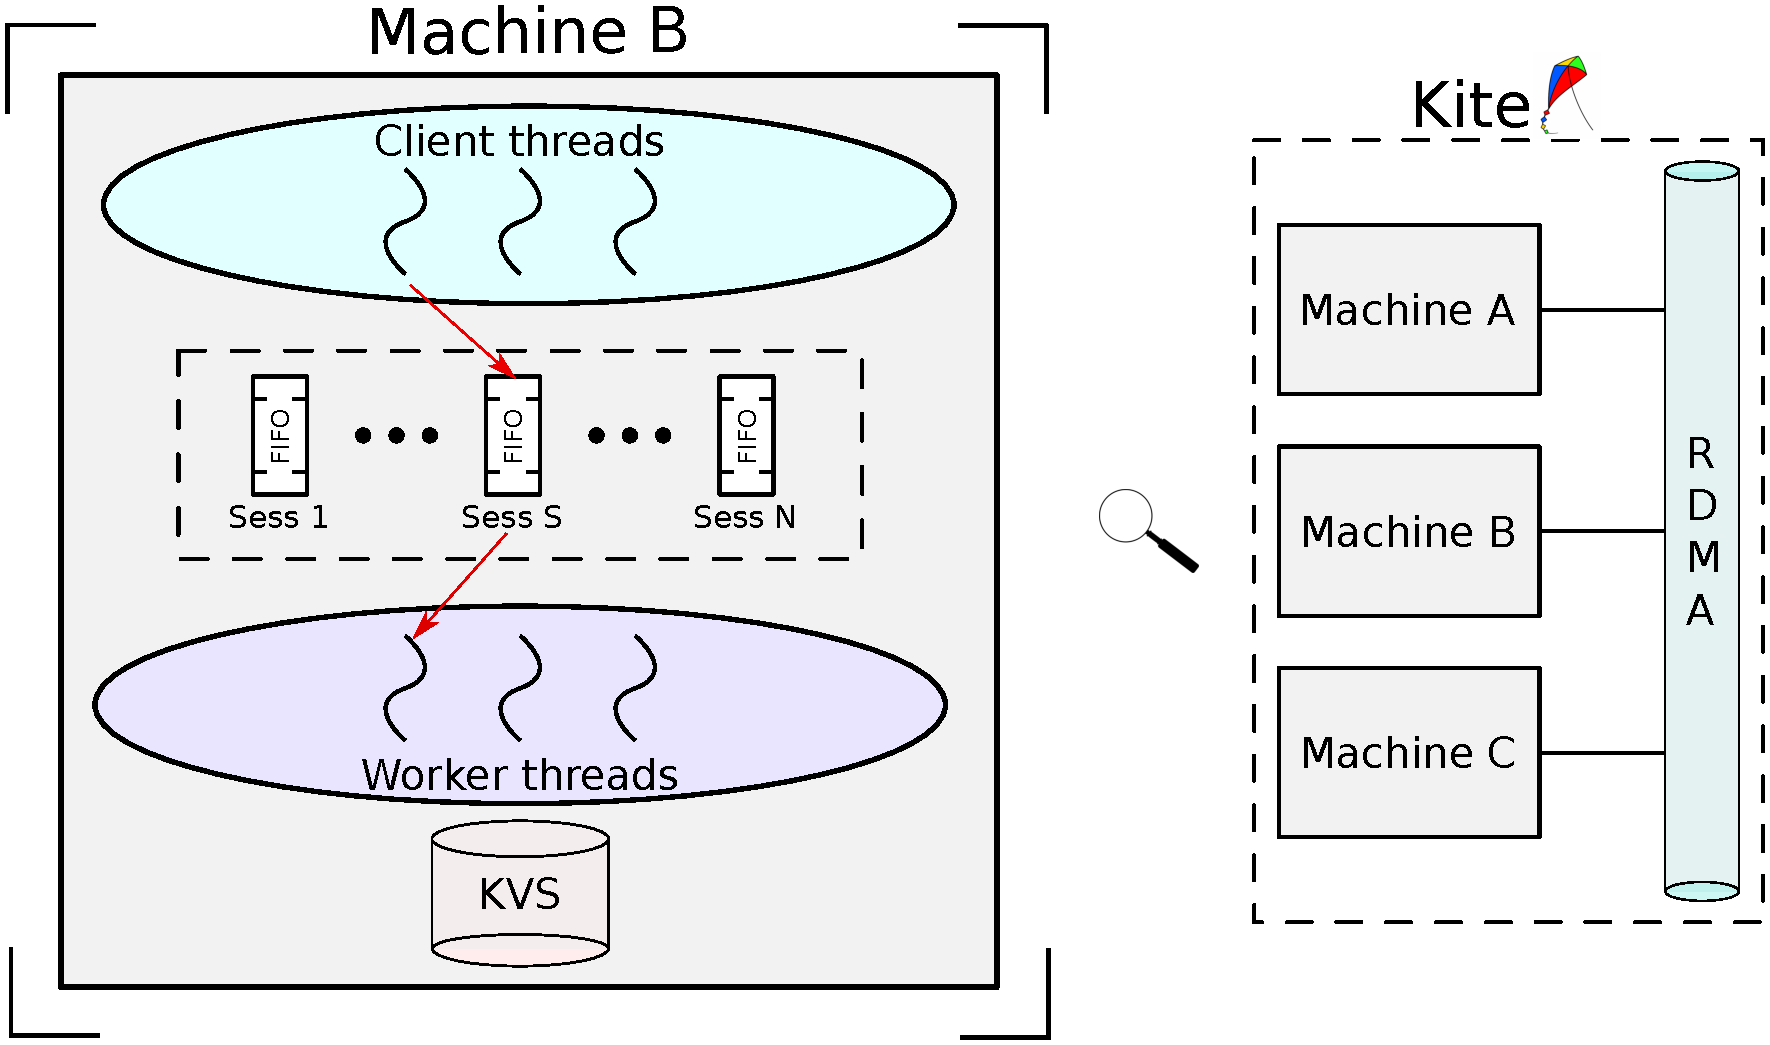
\includegraphics[scale=0.25]{1_figures/Wrkr-clt-Interface.pdf}
%   \vspace{-0.5em}
  \caption{A Kite machine is composed of worker and client threads, that interface through the session FIFOs.}
%   \vspace{-1.5em}
  \label{fig:interface}
\end{figure}


The \odlib~API offers reads, plain writes, and two types of conditional writes: 1) Fetch-\&-Add (FAA), and 2) Compare-\&-Swap (CAS).
%: a weak variant that can complete locally if the comparison fails locally, and a strong variant that always checks remote replicas.  
The \odlib~API includes an asynchronous (\emph{async}) and a synchronous (\emph{sync}) function call for every request (similarly to Zookeeper~\cite{Hunt:2010}). 


\beginbsec{Synchronous API } 
A sync call issues the request and then blocks polling for the request's completion.
We provide here the function call that issues a sync read:
\begin{lstlisting} 
sync_read(key_id, val_len, *value_ptr, session_id)
\end{lstlisting}
The programmer provides the key to be read ($key\_id$), the size of the value in bytes ($val\_len$), a pointer where the value should be copied ($*value\_ptr$) and the session id ($session\_id$). The call returns an integer, which, if 
negative, maps to an error code.
Sync calls simplify programming, but are not very efficient, as the client may need to block for several microseconds waiting for a request to complete. 

\beginbsec{Async API } An async call returns immediately before the request has completed. The client can call a polling function to find out if the request has been completed. As an example, we provide here the async read call:
\begin{lstlisting} 
async_read(key_id, val_len,  *value_ptr, session_id)
\end{lstlisting}
The call returns an integer, which, if negative, maps to an error code; otherwise, the returned integer denotes the \emph{request id} that can be used by the client to poll for the request's completion. \odlib~provides a range of  polling functions, that typically require a session id and a request id as arguments. 
\end{comment}
\begin{comment}
\beginbsec{Batched Asynchronous Programming }
Despite its performance benefits, an asynchronous API is admittedly quite cumbersome to program with.
For that reason, we make the following simplification: completed requests can only be polled in session order, irrespective of the order in which the worker completes them. This enables the client thread to issue a batch of requests and then at a later time, poll only for the last request issued.
If the last request is successfully polled, it guarantees that all preceding requests have been completed. We found this pattern very natural in porting code to \odlib.



\beginbsec{Multiple sessions per client thread} 
A client thread can use multiple sessions to improve performance: enabling thread-level parallelism across the workers, and session-level parallelism within one worker thread. 
Programmers can leverage this feature to parallelize their applications, by allocating parallelizable
tasks to different sessions. We leverage this capability when porting lock-free data structures to \odlib, 
in order to allow clients threads to work on multiple distinct operations concurrently, through different sessions. 


\beginbsec{Session FIFO}
Session FIFOs constitute the communication medium between client and worker threads. There can be thousands of sessions FIFOs (one per session), where each session maps to exactly one client and one worker thread. Therefore, any given session FIFO can only be accessed by one worker and one client. 
We focus on one slot of a single session FIFO. 
The slot's fields are illustrated in Figure~\ref{fig:fsm}a. The client fills the fields of the slot to issue a request, and the worker uses the fields to complete the request. For instance, on a CAS request the worker writes the result in the \emph{rmw result} field. If the CAS is unsuccessful, the worker also writes the read value in the address pointed to by the \emph{read value ptr} field.


\beginbsec{Request FSM} A FIFO slot contains a \emph{state} variable, which is used to facilitate the synchronization between worker and client. The state variable works as an Finite State Machine (FSM) (Figure~\ref{fig:fsm}), transitioning between four possible states, denoting who can access the slot. A client issues a request to the slot only if the state is \emph{Invalid}; issuing the request transitions the state to \emph{Active}, which implicitly passes the ownership of the slot to the worker thread. The worker will transition the slot to \emph{In-progress} when it polls it and later to \emph{Completed} when it completes it.


\begin{figure}[t]
   \centering
  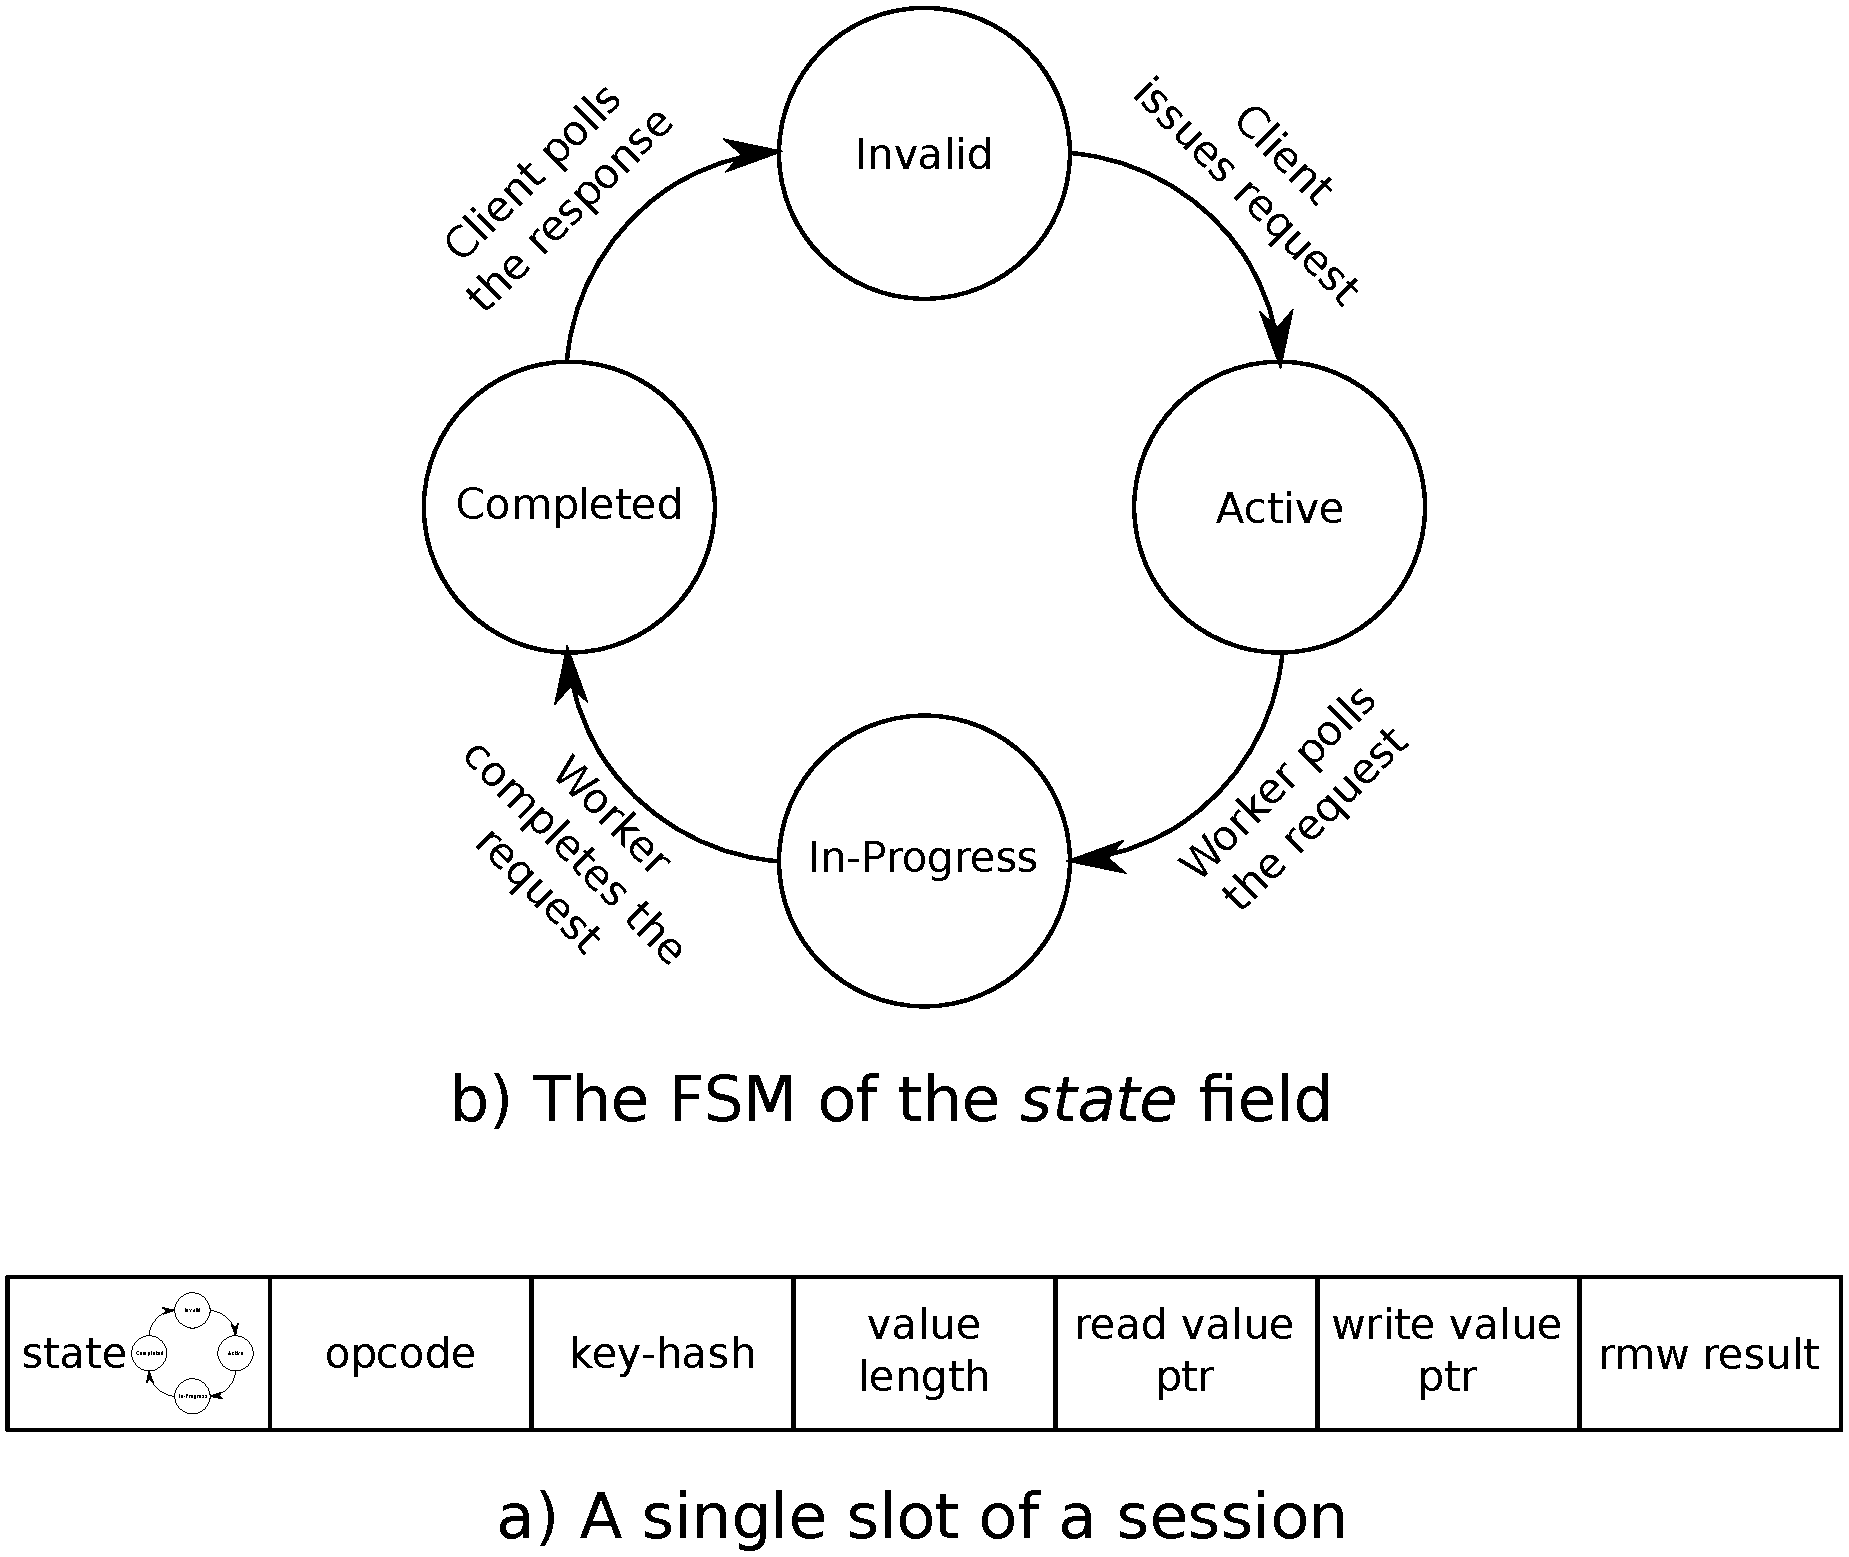
\includegraphics[scale=0.25]{1_figures/state-FSM.pdf}
  %\vspace{-1.5em}
  \caption{The fields of one slot of one session FIFO, and the FSM of the state field.}
  \label{fig:fsm}
\end{figure}
\end{comment}